\documentclass{article}

\usepackage{graphicx}
\usepackage{tikz}
\usepackage{tikzsymbols}
\usetikzlibrary{calc,patterns,shapes.geometric}
\pagestyle{empty}
\usepackage[margin=0pt]{geometry}
\geometry{papersize={14in,12in}}

\def\centerarc[#1](#2)(#3:#4:#5){\draw[#1] ($(#2)+({#5*cos(#3)},{#5*sin(#3)})$) arc (#3:#4:#5);}

\begin{document}
	\begin{figure}
		\centering
		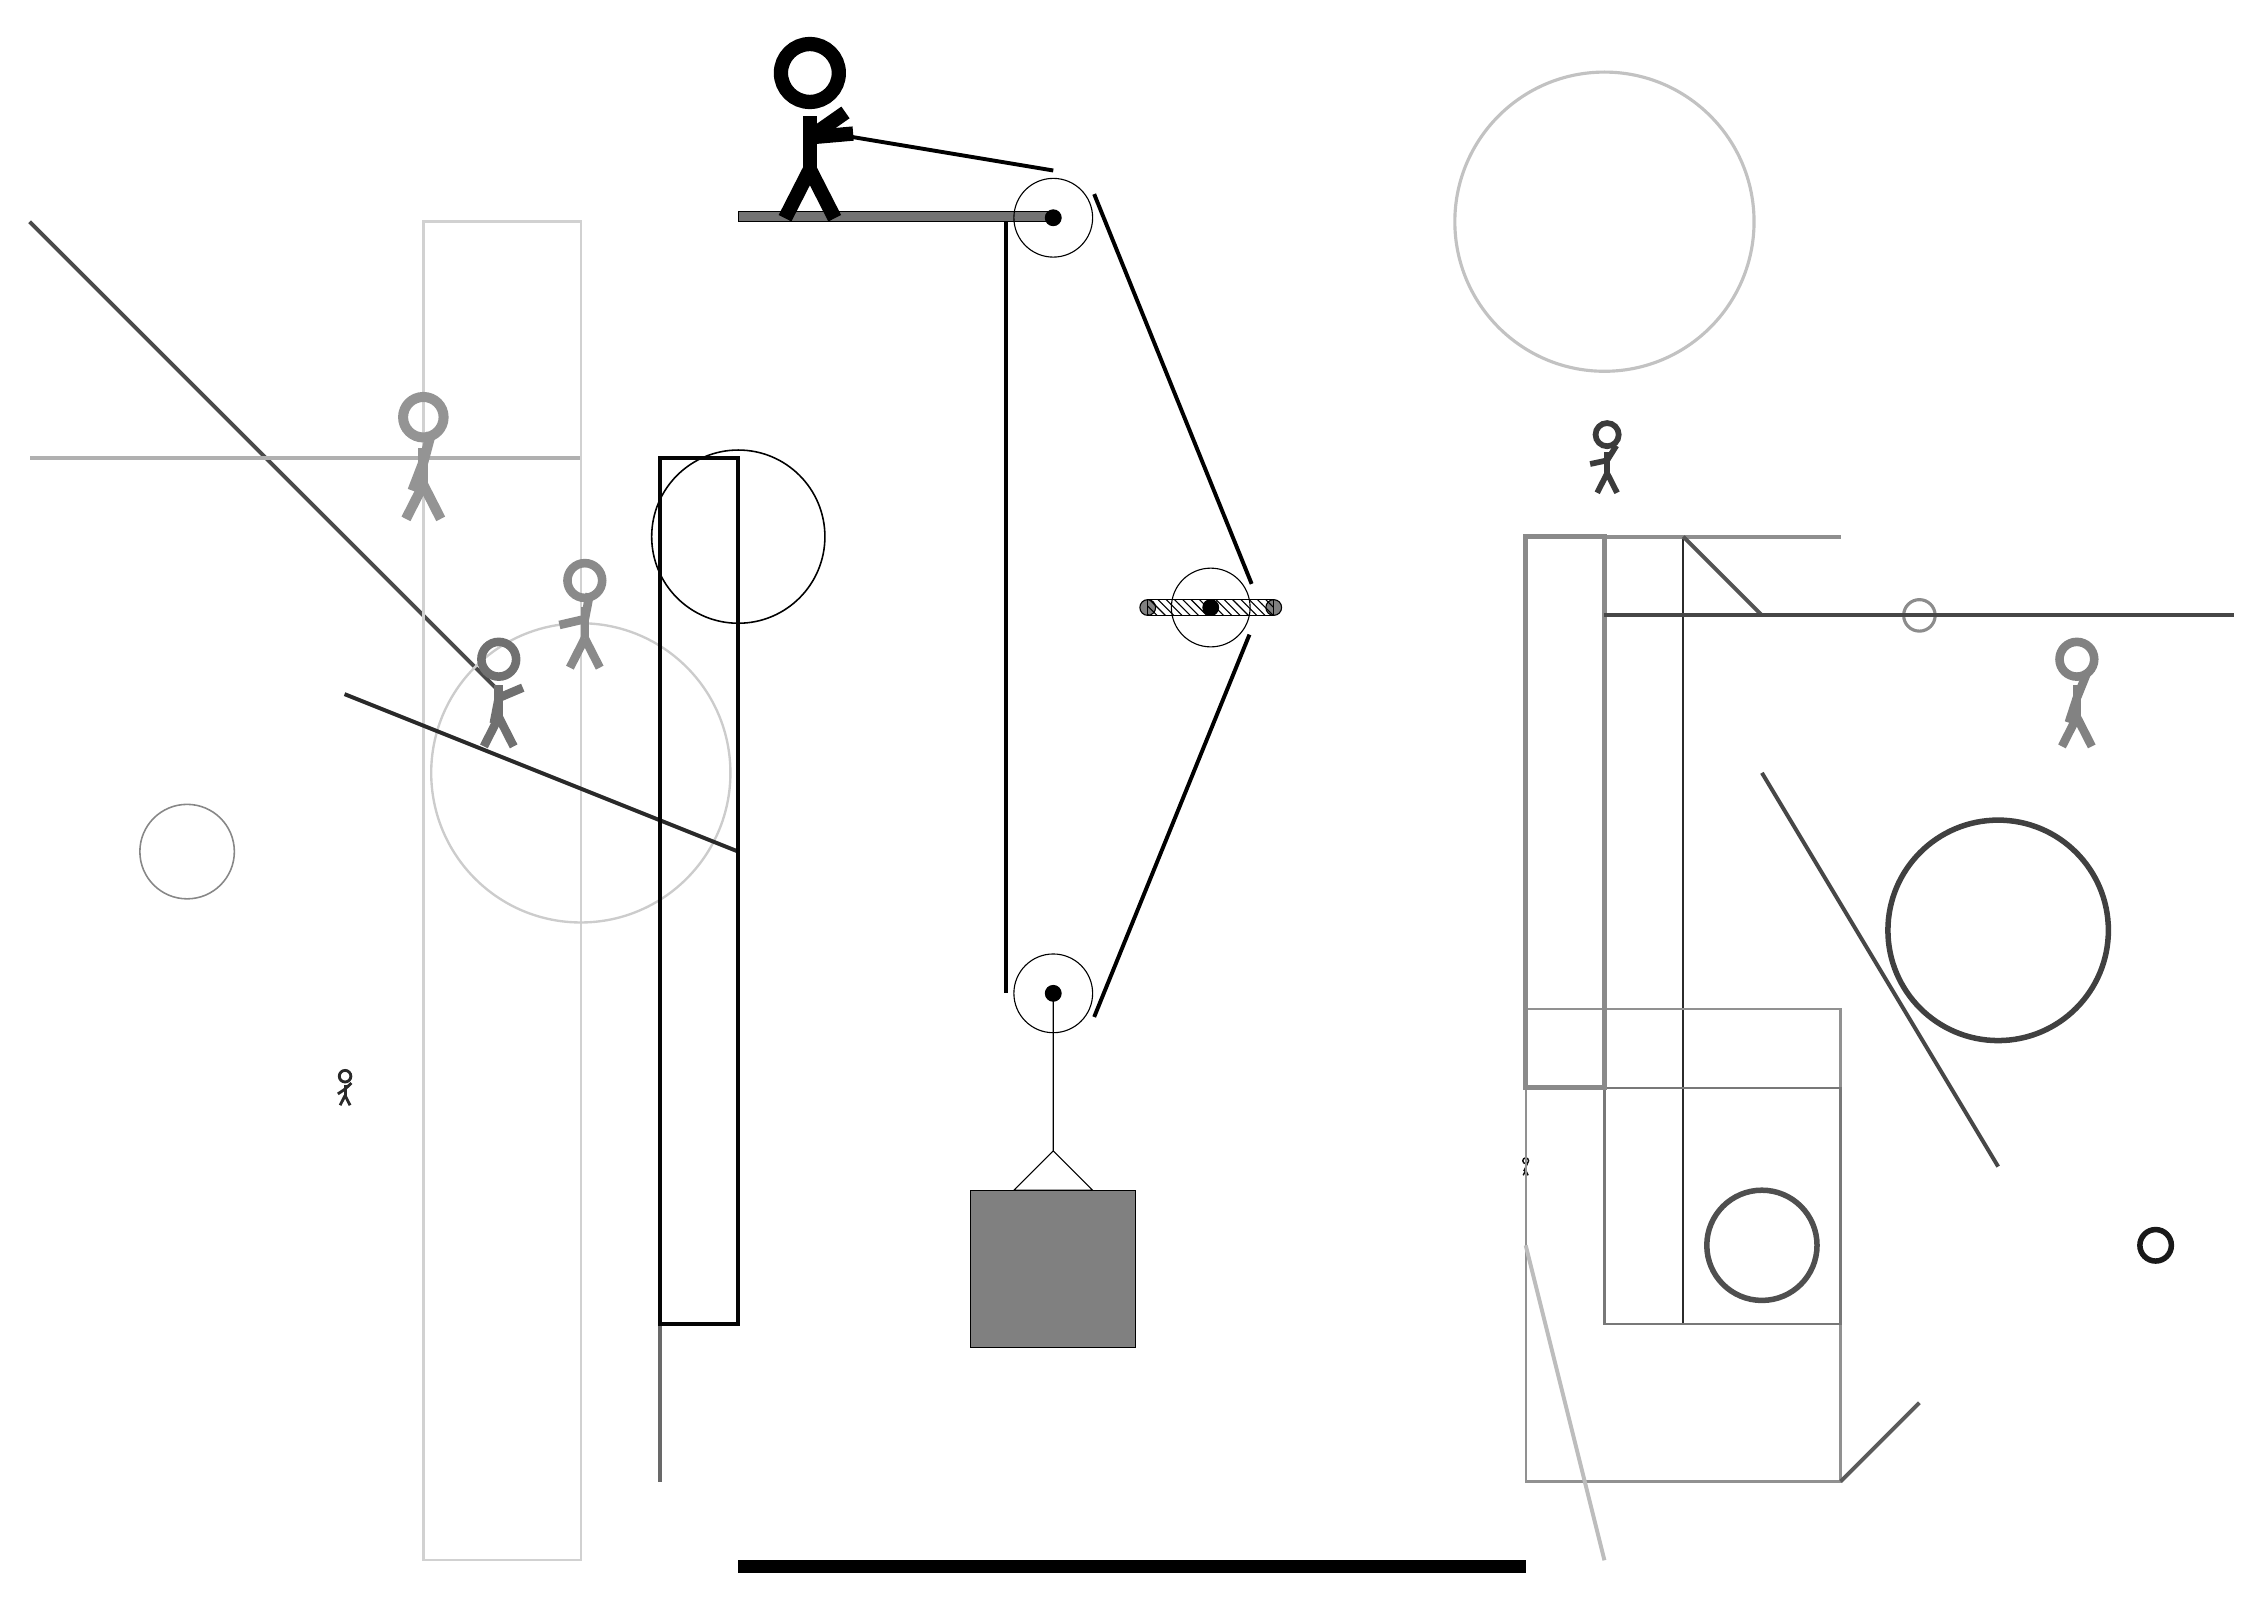
\begin{tikzpicture}
			%%%%% START %%%%%
			
			\draw[fill=black!55] (-2, 14) rectangle (2, 14.125);
			
			\draw (2, 4.2) circle (0.5);
			\draw[fill=black] (2, 4.2) circle (0.1);
			
			\draw (2, 14.05) circle (0.5);
			\draw[fill=black] (2, 14.05) circle (0.1);
			
			\node[line width=0.7mm, color=black!94] at (8, 2) {\Strichmaxerl[1][64][65]};
			
			\node[line width=0.3mm, color=black!84] at (-7, 3) {\Strichmaxerl[2][34][44]};
			\draw[line width=0.3mm, color=black!83] (10, 10) rectangle (9, 0);
			\draw[line width=0.5mm, color=black!71](-5, 8) -- (-11, 14);
			\draw[line width=0.5mm, color=black!31](-4, 11) -- (-11, 11);
			
			\draw[line width=0.5mm, color=black!44](9, 10) -- (12, 10);
			\draw[line width=0.3mm, color=black!18] (-4, -3) rectangle (-6, 14);
			\draw[line width=0.3mm, color=black!43] (8, -2) rectangle (12, 4);
			\draw[line width=0.5mm, color=black!64](12, -2) -- (13, -1);
			\draw [line width=0.3mm, color=black!20](-4, 7) circle (1.9);
			\draw[line width=0.5mm, color=black!59](-3, 3) -- (-3, -2);
			
			\draw [line width=0.7mm, color=black!69](11, 1) circle (0.7);
			\node[line width=0.6mm, color=black!49] at (15, 8) {\Strichmaxerl[6][72][68]};
			\draw[line width=0.5mm, color=black!72](11, 7) -- (14, 2);
			\node[line width=0.6mm, color=black!42] at (-6, 11) {\Strichmaxerl[7][69][75]};
			\draw [line width=0.4mm, color=black!24](9, 14) circle (1.9);
			
			\node[line width=0.3mm, color=black!46] at (-4, 9) {\Strichmaxerl[6][13][79]};
			
			\node[line width=0.2mm, color=black!56] at (-5, 8) {\Strichmaxerl[6][79][23]};
			\draw [line width=0.7mm, color=black!90](16, 1) circle (0.2);
			\draw[line width=0.5mm, color=black!26](8, 1) -- (9, -3);
			\draw [line width=0.4mm, color=black!45](13, 9) circle (0.2);
			
			\draw[line width=0.5mm, color=black!67](11, 9) -- (10, 10);
			
			\draw [line width=0.2mm, color=black!100](-2, 10) circle (1.1);
			\draw [line width=0.2mm, color=black!47](-9, 6) circle (0.6);
			\draw[line width=0.3mm, color=black!53] (9, 0) rectangle (12, 3);
			
			\node[line width=0.3mm, color=black!77] at (9, 11) {\Strichmaxerl[4][12][58]};
			\draw[line width=0.6mm, color=black!46] (8, 10) rectangle (9, 3);
			\draw[line width=0.5mm, color=black!84](-7, 8) -- (-2, 6);
			\draw[line width=0.5mm, color=black!72](9, 9) -- (17, 9);
			\draw [line width=0.7mm, color=black!75](14, 5) circle (1.4);
			\draw[line width=0.5mm, color=black!98] (-2, 11) rectangle (-3, 0);
			
			\draw[fill=white](4, 9.1) circle (0.5);
			\draw[fill=black] (4, 9.1) circle (0.1);
			\draw[fill=black!50] (3.2, 9.1) circle (0.1);
			\draw[fill=black!50] (4.8, 9.1) circle (0.1);
			\draw[pattern=north west lines, pattern color=black] (3.2, 9.2) rectangle (4.8, 9.0);
			
			\draw (2, 4.2) -- (2, 2.2) -- (1.5, 1.7) -- (2.5, 1.7) -- (2, 2.2);
			\draw[fill=black!50] (0.95, 1.7) rectangle (3.05, -0.3);
			
			\draw[line width=0.5mm] (1.4, 14) -- (1.4, 4.2);
			\centerarc[line width=0.5mm](2, 4.2)(180:330:0.6);
			\draw[line width=0.5mm](2.5196, 3.9) -- (4.4915, 8.7558);
			\centerarc[line width=0.5mm](4, 9.1)(390:325:0.6);
			\draw[line width=0.5mm](4.5196, 9.4) -- (2.5196, 14.35);
			\centerarc[line width=0.5mm](2, 14.05)(30:90:0.6);
			\draw[line width=0.5mm](2, 14.65) -- (-1, 15.15);
			
			\node at (-1, 15.15) {\Strichmaxerl[10][-175][35]};
			
			\draw[fill=black] (-2, -3) rectangle (8, -3.15);
			
			%%%%% END %%%%%
		\end{tikzpicture}
	\end{figure}	
\end{document}